%% ------------------------------------------------------------------------- %%
\chapter{Desenvolvimentos e resultados} %Nome do capítulo.
\label{cap:resultados} %Rótulo para futura referência ao capítulo. Em qualquer lugar da tese, você poderá citar este capítulo através de ~\ref{cap:introducao}. Você escolhe o argumento de \label e pode ser qualquer coisa (Ex: \label{Procedimento_Experimental})
Os resultados explicitados nesta dissertação estão focados no processamento de 
áudio através de códigos em liguagens de programação de computadores e
voltado para a música e na síntese de estruturas musicais. O tema é amplo
e pertinente o suficiente para contar atualmente com ampla bibliografia e um histórico
que remonta desde a própria história da computação e das linguagens de programação.
Desta forma, entendemos cabível focar este texto nas empreitadas realizadas pelos autores
da presente dissertação, com foco nas realizações do primeiro autor. São usos
reais destas tecnologias, manifestadas de forma cultural e com repercussões
sociais, como poderá é relatado neste mesmo capítulo.

Tais realizações possuem um espectro amplo
dentro do escopo proposto e constitui um percurso relativamente completo
pelas possibilidades e decorrências da abordagem da música pelo código computacional\footnote{ao menos dentro do se denomina 'Cultura Livre', veja o primeiro capítulo do presente escrito para maiores informações}.

Estaremos abordando experimentos abertos em áudio, abordagens musicais pelo código, incluindo música em tempo real, diferido, na matéria e repercussões no tecido social. De forma a relatar os resultados destas investidas, segue uma sessão sobre ações coletivas realizadas através das mobilizações que estes códigos criaram, e as estruturas virtuais mantidas na intenet relacionadas a estas mobilizações e ações. Por fim, alguns materiais didáticos criados pelo autor - que possuem algum papel emblemático - são também expostos por comporem o arsenal de repercussões desta investida no em som e código. 

  \section{Experimentos abertos em áudio: LADSPAs, Wavelets e Redes Complexas}

Todos os desenvolvimentos desta dissertação estão em repositórios abertos\cite{repositorios-tese-dev}.
Alguns foram especialmente importantes como percurso para o que é apresentado neste
escrito. Ou seja, são explorações que manifestaram diferentes aspectos
do trabalho do código voltado para o áudio e a música.

O código para a arte sonora, incluindo a musical, manifesta-se como cultura pois é fruto de práticas
espontâneas, diárias e coletivas.
\footnote{As chamadas culturas biopunk, ciberpunk, cipherpunk, hacker, digital e outras mais,
possibilitadas aos recentes desenvolvimentos em telecomunicação, dizem respeito em menor
ou maior grau à produção de código como cultura.}

A seguir apresentamos alguns bons exemplos dos desenvolvimentos
desta dissertação especificamente em áudio, sem o envolvimento direto da música. São
códigos de necessidade para música, mas de uso mais geral e cuja implementação
requer muito mais de processamento de sinais e computação do que de música propriamente dito.

      \subsubsection{Plugins LADSPA e lv2}
      [repos AE, LM, wiki EL, historico CDTL]
LADSPA (Linux Audio Developers Simple Plugin API) é a API livre\footnote{Veja o Capítulo 1 para a definição de livre neste contexto.} estabelecida de plugins de áudio até a presente data. A última versão liberada desta API é a 1.1, em uso corrente até hoje e é de 2002 segundo os arquivos de cabeçalho relacionados.

A exploração de APIs específicas foge ao escopo do presente texto e os códigos completos podem ser encontrados pela rede, junto a tutoriais e plugins de exemplo. O código destes desenvolvimentos e pertinente ao áudio são relativos à síntese e remoção de ruídos. Da síntese, exitem abordagens mais puristas, que no caso sintetiza ruído branco e filtra para resultar nos espectros desejados (veja logo abaixo para maiores especificações). Uma abordagem menos purista porém mais eficiente é a de usar uma amostra curta do ruído e reproduzí-la indefinidamente através de \emph{cross-fades}.

Já na remoção de ruídos as abordagens são as mais variadas e extremamente dependentes da aplicação. A complexidade dos algorítmos pode atingir níveis de especialidade em processamento de sinais que merecem um trabalho dedicado. Aqui iremos expor somente sobre remoção de ruído \emph{'Hum'} causado usualmente pela corrente alternada que alimenta os equipamentos utilizados.

Abaixo dispomos explicações breves sobre os diferentes ruídos e os códigos relacionados. Preferimos expor em Python os códigos de síntese
por questão de clareza e coerência com o resto do texto\footnote{Os códigos em C/C++ e a implementação como plugin lv2 está no repositório git LV2 como pode ser visto em: http://labmacambira.git.sourceforge.net/git/gitweb-index.cgi}.

O procedimento de reprodução do ruído através de uma amostra repetida e em crossfade é a seguinte:

[código da reprodução do ruído em loop e croos-fade ~10 linhas]

Sintetizando diferentes ruídos\footnote{Dado o propósito do texto e da implementação, utilizamos nomenclaturas utilizadas na música para os ruídos, como se pode notar.}:
\begin{itemize}
    \item Ruído Branco: 
    \item Ruído Rosa:
    \item Ruído Marrom:
    \item Ruído Violeta:
    \item Ruído Azul:
    \item Ruído Violeta:
    \item Ruído Cinza:
    (nao oficiais)
    \item Ruído Vermelho:
    \item Ruído Laranja:
    \item Ruído Preto:
    \item Ruído Branco Ruidoso:
    \item Ruído Preto Ruidoso:
    \item Clicks:
\end{itemize} 

A remoção de ruído Hum é baseada em uma sequência de filtros notch (ver fundamentos) idealmente dispostos nos harmônicos da frequência de oscilação da corrente elétrica. Cada um destes filtros deve permitir ajustes finos no fator de qualidade e também na frequência central pois trata-se de um sistema real passivel dos mais diversos efeitos de distorção do modelo ideal. Abaixo expomos o código em Python para tal \emph{removedor de ruído} como é chamado. O código C/C++ e a implementação como plugin está no mesmo repositório disponibilizado para a síntese de ruídos.

[código e explicação do remodedor de ruído Hum]


      \subsubsection{Protocolo de compactação de áudio via wavelets, polinômios e permutações}
Criado por Rafael Santos Mendes em conjunto com o primeiro autor deste trabalho e em decorrência do mestrado de André Luvizotto, este método
consiste em aproximar cada folha de uma decomposição WaveletPacket por um polinômio e uma permutação. A permutação facilita a aproximação polinomial, pois leva folhas WP de coeficientes ordenados para sucessões melhor comportadas de seus valores\footnote{O método é descrito em um artigo de 2009: Compressão de Áudio via Wavelets, Aproximações Polinomiais e Permutações [Fabbri, Mendes]}.
Representamos cada permutação por um conjunto ordenado de números inteiros. Já o polinômimo possui poucos coeficientes (usualmente 6 ou 8) e os representamos como um conjunto ordenado de variáveis de tipo ponto flutuante.


      \subsubsection{Processamento de voz via redes complexas}
Conversar com Chu e com Luciano e decidir se retiro esta sessão ou mantenho.

      [codigos bem comentados no audio experiments. Apresentação do trabalho "Speech Polarity Detection using Complex Networks Measures: First Explorations no Complenet de 2010"]



\section{Música no Som Digitalizado}

%\subsection{Caracterização da nota musical discretizada}
\subsection{Caracterização da nota musical}
%\subsection{Caracterização da nota musical digital}
A música é tradicionalmente pensada através de unidades chamadas notas. Em sua concepção
simples, as notas possuem ao menos duração, volume, altura e timbre. Embora estas
sejam características psicofísicas, podemos lidar com elas através de suas características
fisicamente mensuráveis.
Em primeiro lugar, estamos tratando diretamente da representação digital do som. Isso em uma
sequência de amostras igualmente espaçadas no tempo. Desta forma, definimos a
frequência (ou taxa) de amostragem $f_a$ como o número de amostras por segundo do áudio digital e
a sequência $T_i=\{t_i\}$ como um conjunto ordenado de amostras reais separadas por $\delta_a=1/f_a$ segundos.


\subsubsection{Duração}
Desta forma, visando uma nota musical de duração $\Delta$,
teremos uma sequência de $ \Delta . f_a $ amostras\footnote{Observe o abuso de notação:
o limite superior de uma sequência é um número natural, mas $ \Delta . f_a $
só satisfaz esta condição em casos muito excepcionais. Procederemos assim por simplicidade. 
Explicitaremos em texto quando for crucial o procedimento relativo à parte fracionária dos índices
ou de seus limites.}:

\begin{equation}
T_{i}^{\Delta}={\{t_i\}}_{i=0}^{\Delta . f_a - 1}
\end{equation}


\subsubsection{Volume}
O volume depende da reverberação e distribuição dos harmônicos - dentre outras medidas psicofísicas~\cite{chowningVolume} - mas num primeiro momento podemos lidar com ele de forma prática e geral através da potência da onda:

\begin{equation}
pot(T_i^{\Delta})=\frac{\sum_{i=0}^{\Delta . f_a -1} t_i^2}{\Delta . f_a}
\end{equation} 

Como o volume final dependerá da amplificação do sinal nos falantes, o mais importante é a potência relativa de uma nota em relação às outras ou de um trecho da música em relação ao resto. As diferenças de volume são medidas em decibeis, que são
calculadas diretamente com as amplitudes, energias ou potências\footnote{Lembrando que, devido à nossa percepção logarítmica,
em um som de volume $v$ a redução da potência $p$ para uma mesma fração $\nu . p $ 
com $\nu \in [0,1]$ é sentido como a mesma diminuição do volume $v-\kappa$ com $\kappa \geq 0$.}:

\begin{equation}\label{decibeis}
V_{dB}=10log_{10}\frac{pot(T^{'}_i)}{pot(T_i)}
\end{equation}

A quantidade adimensional é denotada pela unidade decibeis ($dB$). A cada 10 $dB$s atribuímos canonicamente
a sensação de "volume dobrado". Importantes resultados de referência são os equivalente em $dB$s de se dobrar
a amplitude ou a potência:

\begin{equation*}
se \quad  t_i^{'}=2 . t_i \quad \Rightarrow \quad pot(T^{'}_i)=4 . pot(T_i) \quad \Rightarrow \quad V^{'}_{dB}=10log_{10} 4 \quad  \approx \quad 6 dB
\end{equation*}
\begin{equation*}
se \quad pot(T^{'}_i)=2 pot(T_i) \quad \Rightarrow \quad V^{'}_{dB}=10log_{10} 2 \quad \approx \quad 3 dB
\end{equation*}

Outro valor de referência é a amplificação necessária para que uma sequência tenha o volume dobrado ($10dB$s a mais):

\begin{gather}
10log_{10}\frac{pot(T^{'}_i)}{pot(T_i)} = 10 \quad \Rightarrow \quad \sum_{i=0}^{\Delta.f_a-1}t^{'2}_i=10\sum_{i=0}^{\Delta.f_a-1}t_i^2=\sum_{i=0}^{\Delta.f_a-1}(\sqrt{10}.t_i)^2 \\
\therefore \quad t^{'}_i=\sqrt{10}t_i \quad \Rightarrow \quad t^{'}_i \approx 3,16t_i
\end{gather}

Estes valores servem de guia para os aumentos e diminuições dos valores absolutos que compõem as
sequências de amostras sonoras que visam atingir efeitos musicais.

Neste ponto, correspondendo a uma partícula musical (uma nota), estabelecemos uma sequência cuja
duração e intensidade conseguimos controlar\footnote{Basta alterarmos o tamanho da sequência para alterarmos
a duração ou multiplicarmos as os elementos da sequência por algum valor normalizador}. 

\subsubsection{Altura\footnote{Com ganho de simplicidade e sem perda de generalidade, considere o índice $i=a/b$ como o inteiro mais próximo da divisão $a/b$.}}

A altura é especificada pela frequência fundamental. A frequência fundamental $f_0$ especifica uma periodicidade temporal
com ciclo de duração $\delta_{f_0} = 1/f_0$. Esta duração multiplicada pela taxa de amostragem $f_a$ resulta no número de amostras
do ciclo $\lambda_{f_0}=f_a . \delta_{f_0} =f_a/f_0$. Evidente que, sendo $T_i^f$ a sequência sonora de frequência fundamental $f=f_0$:
    
\begin{equation}\label{periodicidade}
     T^f_i=\{ t_i^f \}=\{ t^f_{i+\lambda_{f}}  \}= \{ t^f_{i+\frac{f_a}{f}} \}
\end{equation}

\subsubsection{Timbre}
Enquanto o período da onda corresponde a uma frequência fundamental, o percurso
da onda sonora dentro do período define um espectro harmônico e portanto
um timbre\footnote{O timbre é uma característica subjetiva e complexa. Fisicamente,
o timbre é multidimensional e dado pelo comportamento temporalmente dinâmico
de energias em componentes espectrais tanto harmônicas quanto ruidosas.  Vale salientar que nem tudo
o que se atribui ao timbre se acha manifesto em diferenças espectrais. Uma mesma nota
possui diferentes matizes espectrais, um mesmo instrumento possui diferentes timbres. Mesmo
assim se fala que uma nota e um instrumento possuem um timbre. Por último, até
aspectos culturais ou circunstanciais alteram nossa percepção timbrística.
Na música, espectros
sonoros com diferenças mínimas resultam em
 timbres com diferenças expressivamente cruciais.
}.

O caso mais simples (e mais importante, como veremos a diante) é o do espectro que consiste somente
de sua própria fundamental $f$. Este é o caso da senóide, frequência em movimento oscilatório puro chamado
movimento harmônico simples. Seja $S_i^f$ uma sequência cujas amostras
$s_i^f$ descrevem uma senóide de frequência $f$:

\begin{equation}\label{senoide}
     S^f_i=\{ s^f_i \}=\Bigl\{ \sin\bigl(2\pi \frac{i}{\lambda_f} \bigr)  \Bigr\} = \Bigl\{ \sin\bigl(2\pi f \frac{i}{f_a}\bigr)  \Bigr\} 
\end{equation}

Onde $\lambda_f=\frac{f_a}{f}=\frac{\delta_f}{\delta_a} \;$ é o número de amostras do período\footnote{Neste ponto já se tem toda a base para música "reduced-fi", ver APÊNDICE ~\ref{APENDICE XX}}.

De forma semelhante, outras formas de onda são utilizadas na música por suas qualidades
espectrais e simplicidade. Enquanto a senóide é um ponto isolado no espectro, estas formas
de onda apresentam cadeias de componentes harmônicos e usos específicos.
As formas de onda especificadas em ~\ref{denteDeSerra}, ~\ref{triangular} e ~\ref{quadrada} são dispostas graficamente na figura ~\ref{fig:formasDeOnda}. 
São as formas de onda artificiais tradicionalmente usadas na música para síntese e controle oscilatório de variáveis, apresentam diversos usos também fora da música.

A dente de serra apresenta todos os componentes da série
harmônica com energia decrescente de $-6dB/oitava$. A sequência de amostras temporais pode ser descrita da seguinte forma:
\begin{equation}\label{denteDeSerra}
     D^f_i=\{ d^f_i \}=\Bigl\{ 2\frac{i\,\%\lambda_f}{\lambda_f} -1 \Bigr\}
\end{equation}

A forma de onda triangular apresenta somente os harmônicos ímpares caindo a $-12dB/oitava$:
\begin{equation}\label{triangular}
     T^f_i=\{ t^f_i \}=\Bigl\{1- \Bigl| 2 - 4\frac{i\,\%\lambda_f}{\lambda_f} \Bigr| \Bigr\}
\end{equation}

A onda quadrada apresenta somente os harmônicos ímpares caindo a $-6dB/oitava$:
\begin{equation}\label{quadrada}
     Q^f_i=\{ q^f_i \}= \left\{
         \begin{array}{l l}
              1 & \quad \text{para} \; \; (i\,\%\lambda_f)   <  \lambda_f /2  \\
              -1 & \quad \text{caso contrário}\\
         \end{array} \right.
\end{equation}

A dente de serra é um ponto de partida comum para a síntese subtrativa pois possui
ambos os harmônicos pares e ímpares e em grande quantidade (alguma filtragem atenuante
é útil nos médios e agudos para que o som ganhe naturalidade e fique mais agradável).
Por este mesmo motivo, os harmônicos atenuados da onda triangular
a faz a mais funcional - dentre as citadas - para ser usada sem nenhum tratamento.

Para citar também um uso possível da onda quadrada, ela pode ser usada em uma síntese
subtrativa que vise imitar um clarinete. Este instrumento também só apresenta os
componentes ímpares do espectro harmônico e a onda quadrada pode convir com sua energia abundante nas altas frequências.



\begin{figure}[h!]
    \centering
    \caption{Formas de onda musicais básicas}
        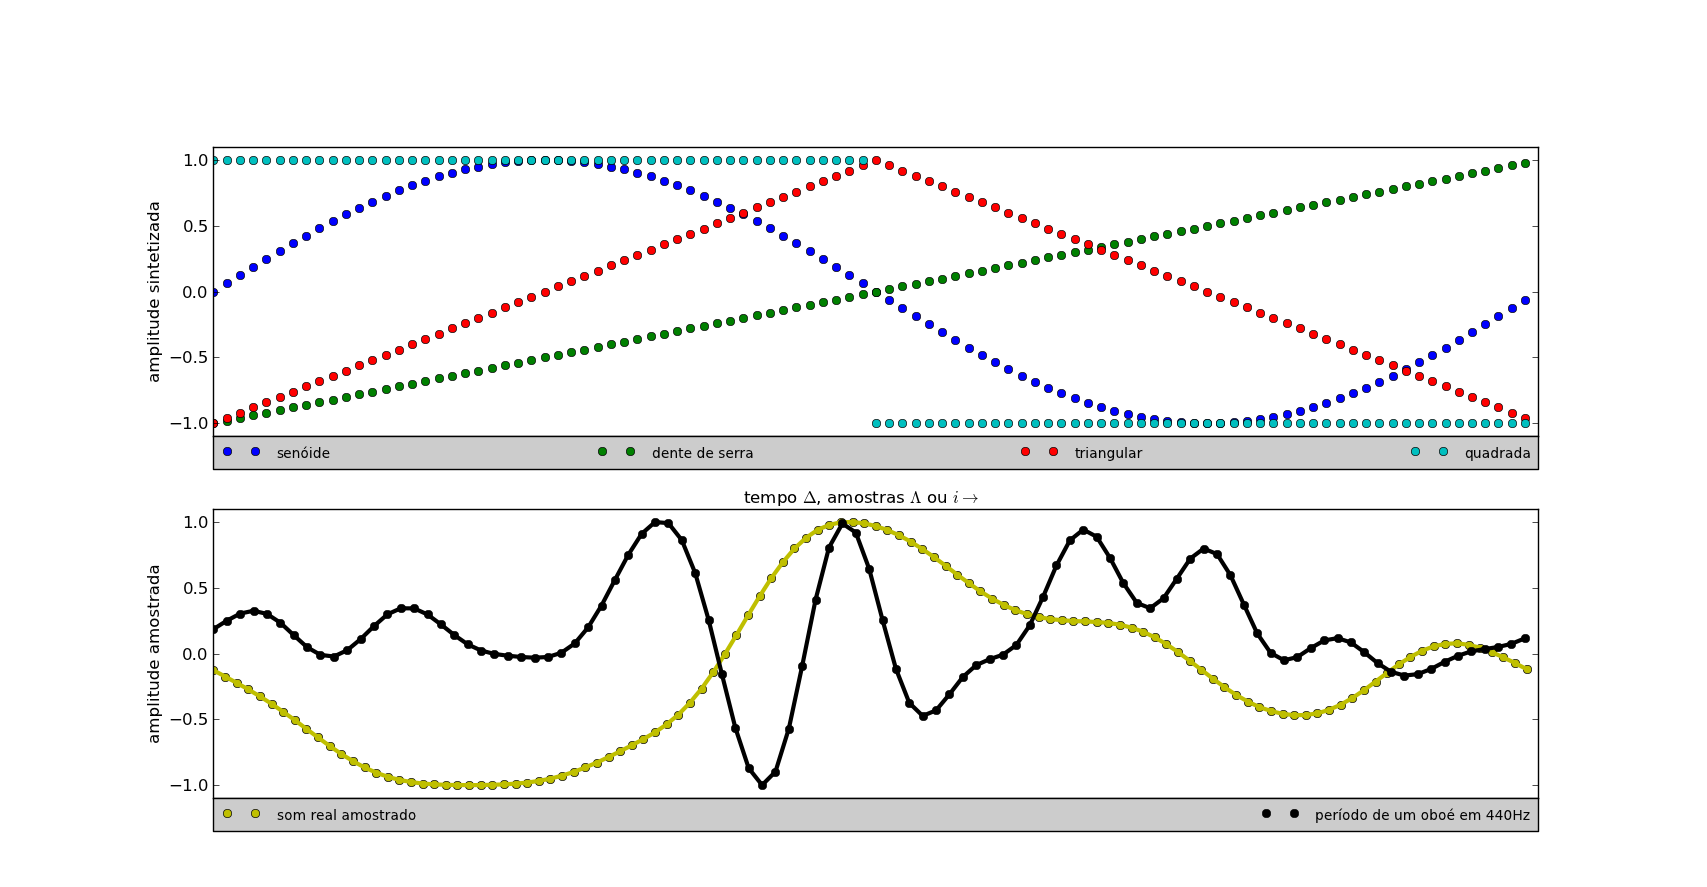
\includegraphics[width=\textwidth]{figuras/formasDeOnda5}
        \label{fig:formasDeOnda}
\end{figure}



A figura ~\ref{fig:formasDeOnda} apresenta
as formas de onda descritas nas equações ~\ref{senoide}, ~\ref{denteDeSerra}, ~\ref{triangular} e ~\ref{quadrada} para $\lambda_f=100$ (período
de $100$ amostras).
Se $t_a=44,1 kHz$, como em padrões PCM e de Compact Disks, a onda possui frequência fundamental $f=\frac{f_a}{\lambda_f}=\frac{44100}{100} = 441 \; Herz $. Um lá\footnote{Um lá 4, logo acima do dó central, no segundo espaço do pentagrama na clave de sol comum.}, seja qual for a forma de onda dentre as artificiais apresentadas.

Estas formas de onda possuem usos especiais na música e seus espectros estão dispostos na figura ~\ref{fig:espectroDeOndas}. É importante notar as componentes isoladas e exatamente harmônicas dos espectros. A senóide consiste de um nódulo único no espectro, frequência pura. A dente de serra é a única com a série harmônica completa (pares e ímpares). Já as ondas triangular e quadrada possuem as mesmas componentes espectrais, mas com decaimentos de $-12dB/oitava$ e $-6dB/oitava$.

\begin{figure}[h!]
    \centering
    \caption{Espectros das ondas sonoras musicais artificiais básicas}
        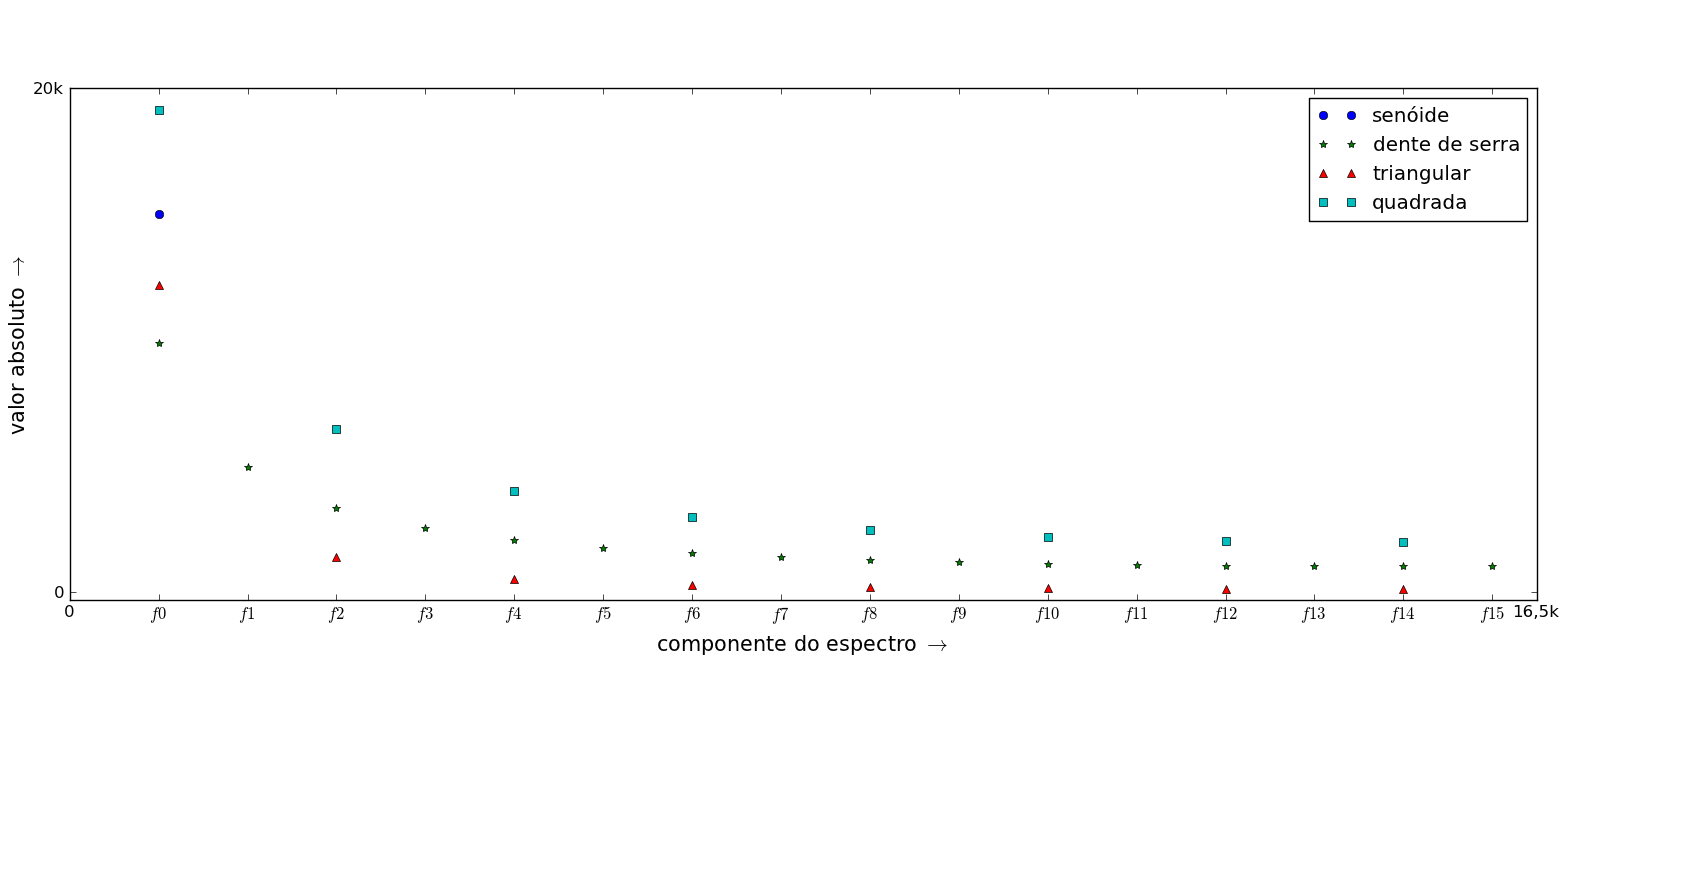
\includegraphics[width=\textwidth]{figuras/espectroDeOndas5}
        \label{fig:espectroDeOndas}
\end{figure}


O espectro harmônico é formado pelas frequências múltiplas da frequência fundamental $f_n=(n+1).f_0$. Como nossa percepção segue a escala logarítmica, o espectro possui notas diferentes da frequência fundamental. Além disso, o número de harmônicos será limitado pela frequência máxima $f_a/2$. 

Musicalmente crucial aqui é internalizar que a presença de
energia\footnote{A energia total equivale à soma dos quadrados das amplitudes como as de pressao/voltagem pelo tempo,e.g. ~\ref{fig:formasDeOnda}.
As componentes espectrais - e.g. ~\ref{fig:espectroDeOndas} e ~\ref{fig:espectroOboe} -
também podem ser elevadas ao quadrado para resultar em quantificação de energia e somam-se na energia total. As energias se equivalem pelo teorema de Parseval.}
em uma componente de frequência $f_n$ na decomposição por fourier 
implica na presença de uma oscilação senoidal na constituição do som, puramente harmônica no som e naquela frequência $f_n$. Esta energia concentrada especificamente na frequência $f_n$ é separada
 pelo ouvido para adentrar em um nível cognitivo de processamento\footnote{Esta separação em frequência é realizada por diversas espécies através de mecanismos similares à cóclea humana.}.
  As componentes senoidáis são geralmente as principais responsáveis pela qualidade chamada timbre e, caso não apresentem proporções harmônicas (relações de pequenos números), são ruídos, i.e. não são notas com frequência fundamental como o lá 4 ($440 Hz$) de nossos exemplos. Além disso, nossa noção de altura absoluta em um complexo sonoro é baseada na semelhança do espectro com a série harmônica.

No caso de uma forma de onda fixa (e de tamanho fixo), o espectro é sempre harmônico e estático. Fixada a frequência fundamental (inverso do comprimento da onda), cada forma de onda é composta de proporções específicas das componentes harmônicas e 
quanto maior a curvatura do trecho na forma de onda, maior a contribuição do trecho para a
concentração de energia nos harmônicos agudos.

Podemos ver isso claramente em sons reais. A onda rotulada como 'som real amostrado' na figura ~\ref{fig:formasDeOnda} é um período extraído de um som real relativamente comportado. Ele possuí $\lambda_f=114$ amostras\footnote{Caso também utilizado diretamente em $f_a=44,1kHz$, é um pouco mais grave que os $441 Hz$ das formas de onda artificiais $\frac{44100}{114}=385,84Hz$.}. A onda de oboé foi amostrada de um lá 4 também em $44,1kHz$. O período escolhido para a amostragem é relativamente curto, com 98 amostras corresponde a $\frac{44100}{98}=450 Hz$. Pode-se perceber o espectro rico em frequências do oboé e o espectro do mais grave do som real. A figura ~\ref{fig:espectroOboe} 
expõe em conjunto o conteúdo espectral da nota original e o resultante da utilização destas amostras.

Note que, definindo $ R_i=\{ r_i \}_0^{\lambda_f-1}$ a sequência de amostras do som real da figura ~\ref{fig:formasDeOnda},
$R_i$ pode ser tomado como base para um som $T_i^f$ da seguinte forma: 

\begin{equation}\label{sampleandoFormaDeOnda}
     T^f_i=\{ t_i^f \}=\Bigl\{ r_{(i\,\%\lambda_{f})} \Bigr\}
\end{equation}

O som resultante possui o espectro momentâneo do som original. Por ser repetido de forma idêntica,
seu espectro é perfeitamente harmônico, sem os ruídos e variações típicas do fenômeno natural. Isso pode ser visto claramente na figura ~\ref{fig:espectroOboe} onde os espectros da nota original do oboé e de uma nota 
artificial - de mesma duração e cujas amostras consistem no mesmo período da figura ~\ref{fig:formasDeOnda} - estão dispostas juntamente. O espectro natural possui variações na frequência dos harmônicos, nas suas intensidades e uma quantidade de ruído. Já a nota cujo período foi amostrado possui espectro perfeitamente harmônico.



\begin{figure}[h!]
    \centering
    \caption{Espectros das ondas sonoras do oboé natural e de período amostrado}
        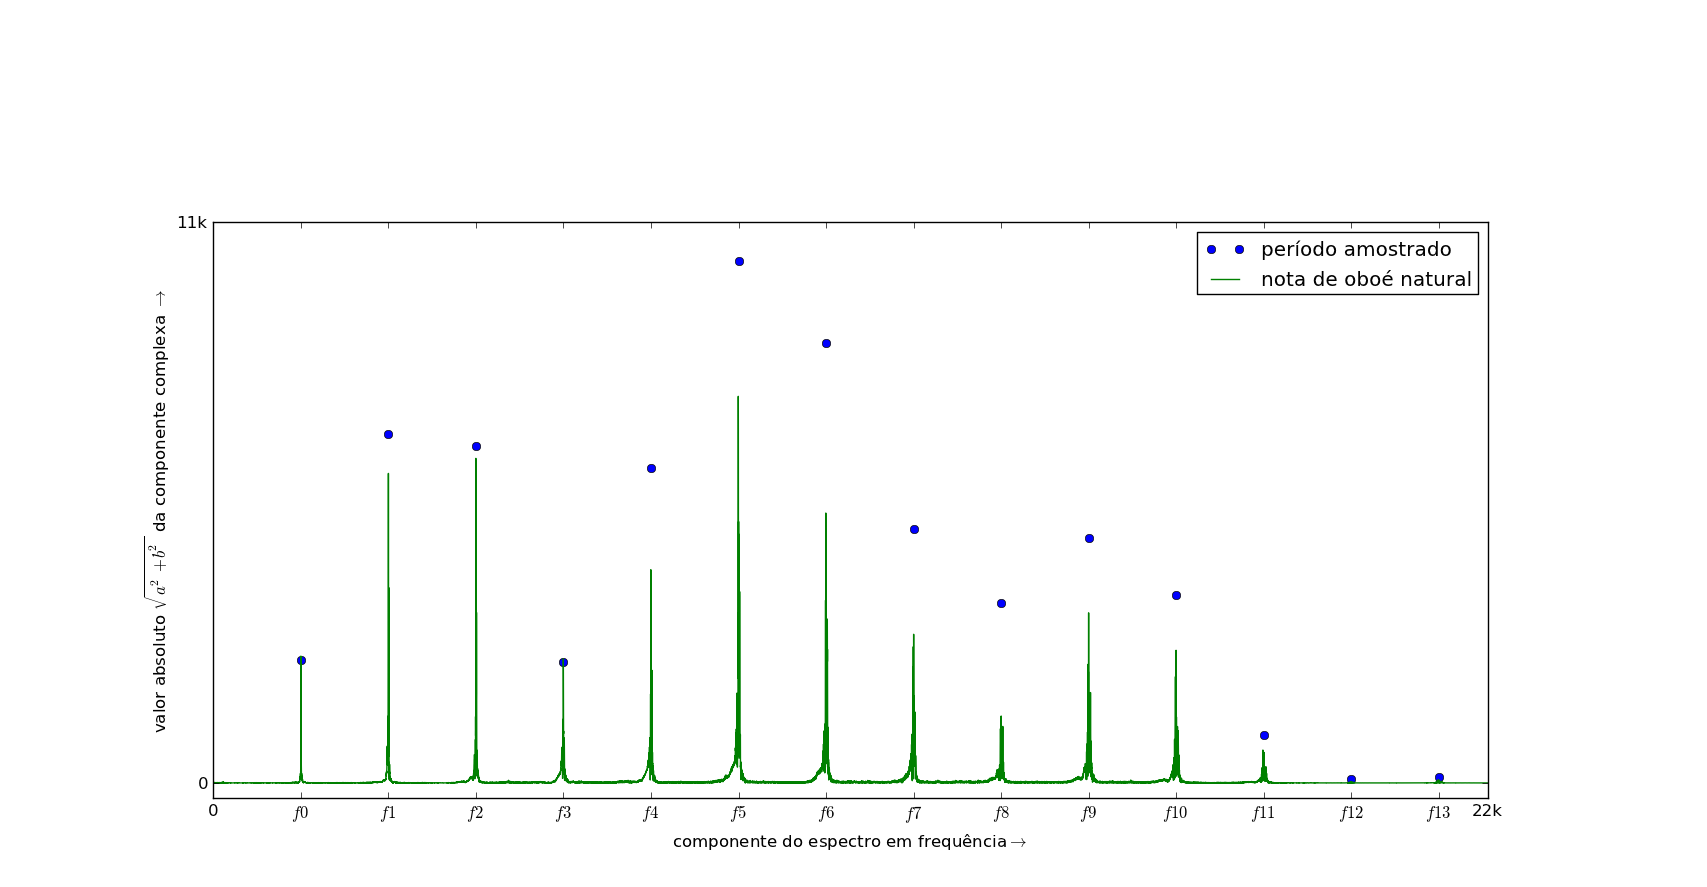
\includegraphics[width=\textwidth]{figuras/espectroOboeAmostradoNatural2}
        \label{fig:espectroOboe}
\end{figure}





\subsubsection{O espectro no som amostrado}
Além deste papel-chave no timbre e na cognição como um todo, a presença e comportamento destas componentes é peculiar no som discretizado. Considere um sinal $T_i$ e sua decomposição de Fourier $\mathcal{F}\{T_i\}=C_i=\{c_i\}_0^{\Lambda-1}$. Sabemos que a recomposição segue a conversão das componentes frequenciais em amostras temporais\footnote{Lembrando que o fator $\frac{1}{\Lambda}$ pode ser distribuído dentre a transformada e a reconstrução como preferir}:

 
\begin{equation}\label{recomposicaoFourier}
t_i = \frac{1}{\Lambda}\sum_{k=0}^{\Lambda-1}c_ke^{j . \frac{2\pi k}{\Lambda} i } = \frac{1}{\Lambda}\sum_{k=0}^{\Lambda-1}(a_k+ j . b_k)\left[cos(w_k i) +j . sen(w_k i)\right]
\end{equation}

Onde $c_k = a_k + j . b_k$ e $w_k=\frac{2\pi k}{\Lambda}$. Nosso som possui amostras $t_i$ reais que resultam das contribuições de cada componente de frequência $w_k$ e cujo $c_k$ regula o módulo e a fase. A parte real da equação ~\ref{recomposicaoFourier} nos fornece a componente de forma mais clara:

\begin{equation}\label{moduloEfase}
\begin{split}
t_i& = \frac{1}{\Lambda}\sum_{k=0}^{\Lambda-1}\left[a_k cos(w_k i) -b_k sen(w_k i)\right] \\
   & = \frac{1}{\Lambda}\sum_{k=0}^{\Lambda-1}\sqrt{a_k^2 + b_k^2} \; cos\left[w_k i - tg^{-1}\left(\frac{b_k}{a_k}\right)\right]
\end{split}
\end{equation}

Podemos notar claramente pela equação ~\ref{moduloEfase} que o termo imaginário apenas acrescenta uma fase à senóide real. Ao mesmo tempo $b_k$ também altera a amplitude mas a informação de amplitude já está em $a_k$, i.e. os termos imaginários da decomposição espectral por Fourier proporcionam a varredura de fase
 $[-\frac{\pi}{2},+\frac{\pi}{2}]$. O sinal de $a_k$ especifica se estamos do lado direito ou esquerdo do circulo trigonométrico, completando a varredura completa de fase (os intervalos $[-\frac{\pi}{2},+\frac{\pi}{2}]$ e $[\frac{\pi}{2},\frac{3\pi}{2}]$ completam $2\pi$).


\begin{figure}[h!]
    \centering
    \caption{Oscilação de 2 amostras (frequência máxima em qualquer $t_a$)}
        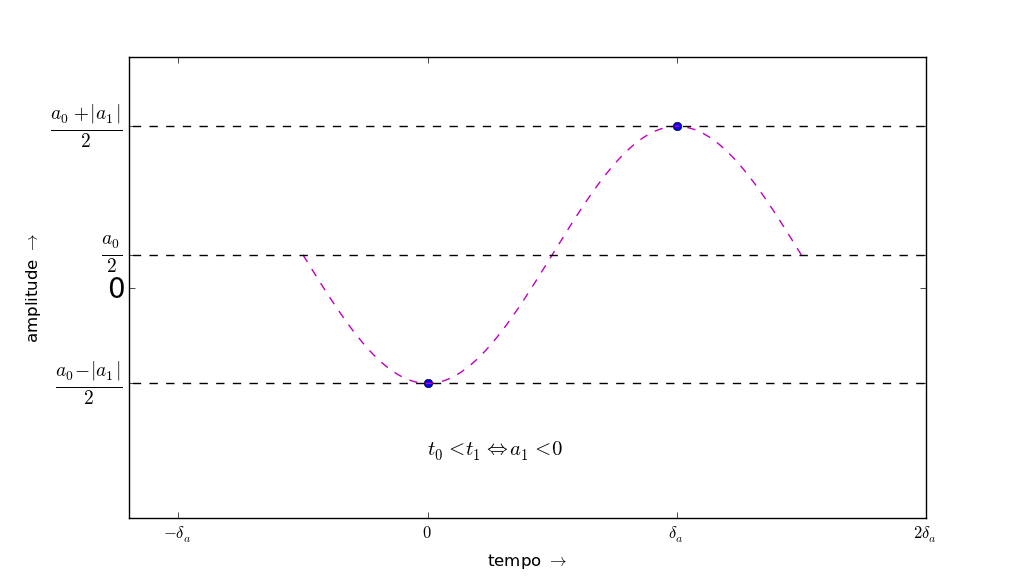
\includegraphics[width=\textwidth]{figuras/amostras2c_}
        \label{fig:amostras2}
\end{figure}

A figura ~\ref{fig:amostras2} exibe duas amostras e a componente espectral que contém. A decomposição de Fourier resulta neste caso em somente dois coeficientes $\{c_k=a_k-j.b_k\}_0^{\Lambda-1=1}$. O papel das amplitudes $a_k$ fica bem claro:
 $a_0$ é controla o deslocamento fixo\footnote{chamado de bias ou offset} e $a_1$ especifica a amplitude da oscilação em si. A frequência que possui a energia\footnote{Lembrando que as energias garantidamente se equivalem pela $\frac{1}{\Lambda} . \sum_{k=0}^{\Lambda -1}c_k^2 = \sum_{i=0}^{\Lambda-1}t_i^2$ (Teorema de Parseval)}
 $e_k=\frac{(c_k)^2}{\Lambda=2}$ é dada pela relação $f_k=k . \frac{f_a}{\Lambda=2} $.  Ou seja, no caso de duas amostras só temos energia nas frequências $f_0=0$ e $f_1=\frac{f_a}{\Lambda=2}=f_{\text{máx}}$.

Este caso é de especial importância pois o mínimo necessário para representar uma oscilação são 2 amostras e disso resulta a frequência de Nyquist $f_{\text{máx}}=\frac{f_a}{2}$. Esta é a frequência máxima presente em um som amostrado com $f_a$ amostras por segundo\footnote{Qualquer sinal amostrado possui esta característica, não somente o som digitalizado.}.

Vejamos o que acontece no caso de 3 amostras. Todas as sequências fixas $T_i$ de apenas 3 amostras também apresentam
somente 1 frequência, pois sua primeira harmônica usaria 1,5 amostras e ultrapassa o limite inferior de 2 amostras mínimas (a frequência da harmônica ultrapassaria a de Nyquist pois:  $\; \frac{f_a}{3}.2 > \frac{f_a}{2} $). Se $\Lambda=3$, 
os coeficiêntes $\{c_k\}_0^{\Lambda-1=2}$ da decomposição por Fourier apresentam-se em 
3 componentes frequenciais. Uma delas é a frequência zero, as outras duas contribuem de forma igual na reconstrução da senóide com $f=f_a/3$.

\begin{figure}[h!]
    \centering
    \caption{3 amostras apresentam uma única frequência}
        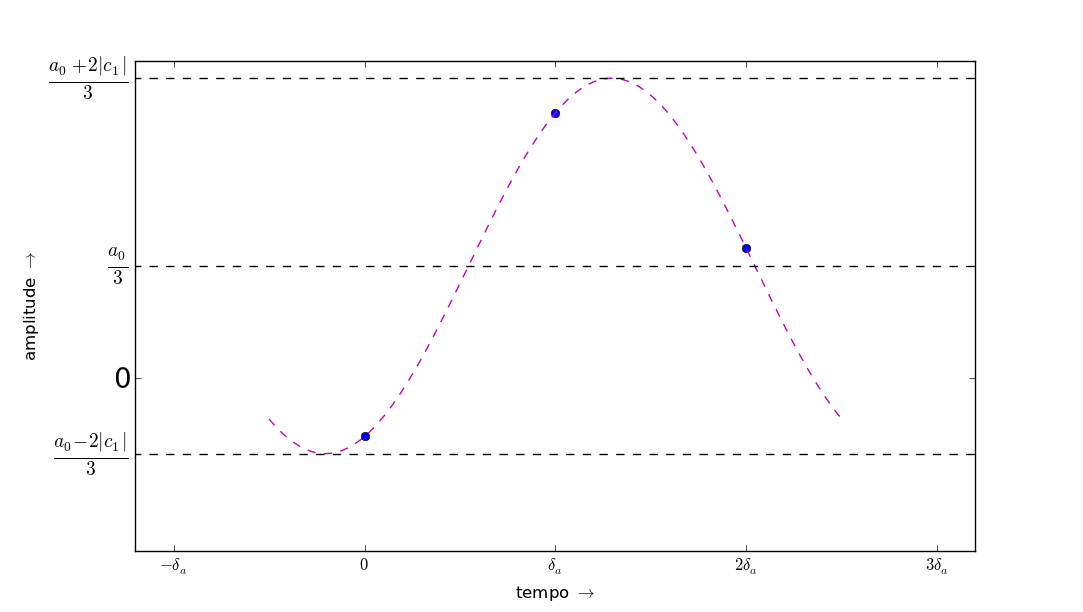
\includegraphics[width=\textwidth]{figuras/amostras3b}
        \label{fig:amostras3}
\end{figure}



Partimos de $\Lambda$ amostras reais $t_i$ e temos $\Lambda$ coeficientes complexos $c_k=a_k+j.b_k$. Os coeficientes $c_k$ se equivalem dois a dois\footnote{Módulos iguais e fases com sinais opostos; $a_{k1}=a_{k2}$ e $b_{k1}=-b_{k2}$.} pois correspondem às frequências $f_k = k.\frac{f_a}{\Lambda}, \; k \in \{0...\Lambda-1\} $
 e quando $ f_k > f_{\text{máx}} = \frac{f_a}{2} $ (o que já exclui $f_0=0$ e $f_k=\frac{f_a}{2}$), a frequência $f_k$ é espelhada para $f_l=\frac{f_a}{2} - (f_k-\frac{f_a}{2})=f_a-f_k=f_a - k\frac{f_a}{\Lambda}=(\Lambda-k)\frac{f_a}{\Lambda} \Rightarrow f_k\equiv f_{\Lambda-k}$. 
 
 O mesmo pode ser observado com 
 $w_k=f_k.\frac{2\pi}{f_a}$ e lembrando da periodicidade $2\pi$, que resulta em $w_k=-w_{\Lambda-k}$. Como o coseno é uma função par e a tangente inversa é impar, as componentes em $w_k$ e $w_{\Lambda-k}$ se somam na equação de reconstrução das amostras reais mostrada em ~\ref{recomposicaoFourier}.

  Dito de outra forma, em uma decomposição de $\Lambda$ amostras, as $\Lambda$ componentes frequenciais $\{c_i\}_0^{\Lambda-1}$ resultantes
   são equivalentes em pares.
   Excepcional excessão para $f_0$ e, no caso de $\Lambda$ ser par, de $f_{\Lambda/2}=f_{\text{máx}}=\frac{f_a}{2}$. Além disso, estas duas frequências (a frequência zero e a frequência máxima) não são representadas com variação de fase e, portanto, são estritamente reais. Assim, podemos 
   concluir que o número $\tau$ de pares de coeficientes equivalentes é:

\begin{equation}\label{coefsPareados}
\tau = \frac{\Lambda - \Lambda \% 2}{2} +\Lambda \% 2 -1
\end{equation}

e resultam evidentes as equivalências ~\ref{equivalenciasFreqs}, ~\ref{equivalenciasModulos} e ~\ref{equivalenciasFases}:

\begin{equation}\label{equivalenciasFreqs}
f_{k}\equiv f_{\Lambda-k}\;, \;\; w_{k}=-w_{\Lambda-k}\;\;\;, \quad \;\; \forall \quad 1 \leq k \leq \tau  
\end{equation}

Como $a_k = a_{\Lambda -k}\;\;$ e $\;\;b_k = - b_{\Lambda -k}$:

\begin{equation}\label{equivalenciasModulos}
\sqrt{a_k^2 + b_k^2} = \sqrt{a_{\Lambda - k}^2 + b_{\Lambda -k}^2} \;\;, \quad \;\; \forall \quad 1 \leq k \leq \tau  \\
\end{equation}

\begin{equation}\label{equivalenciasFases}
tg^{-1}\left(\frac{b_k}{a_k}\right)=-tg^{-1}\left(\frac{b_{\Lambda -k}}{a_{\Lambda - k}}\right)\;\;,\quad \;\; \forall \quad 1 \leq k \leq \tau
\end{equation}


Com $k \in \mathbb{N}$. A observação da equação de reconstrução para o sinal real ~\ref{moduloEfase} em conjunto com as equivalências dos módulos e fases ~\ref{equivalenciasModulos} e ~\ref{equivalenciasFases}
mostra a combinação em fase das componentes em $w_k$ e $w_{\Lambda-k}$:

\begin{equation}
t_i = \frac{a_0}{\Lambda} + \frac{2}{\Lambda}\sum_{k=1}^{\tau}\sqrt{a_k^2 + b_k^2} \; cos\left[w_k i - tg^{-1}\left(\frac{b_k}{a_k}\right)\right]+ \frac{ a_{\Lambda/2+1}}{\Lambda}.(1-\Lambda\% 2)
\end{equation}

Assim, a exemplo da figura ~\ref{fig:amostras3}, a transformada de Fourier de 3 amostras possui 2 coeficientes imaginários que possuem quantidades iguais de energia na mesma frequência.

Com 4 amostras, podemos representar 1 ou 2 frequências em proporções diferentes. A figura ~\ref{fig:amostras4} mostra uma forma de onda de 4 amostras e suas duas componentes. Note que as contribuições individuais se somam de fato na forma de onda original, e que as curvaturas maiores são fruto da frequência mais aguda.

A figura ~\ref{fig:formas4} explicita os harmônicos em 4 amostras nas formas de onda básicas das equações ~\ref{senoide}, ~\ref{denteDeSerra}, ~\ref{triangular} e ~\ref{quadrada} e figura ~\ref{fig:formasDeOnda}. Todas consistem em apenas 1 senóide, com excessão da dente de serra que possui os harmônicos pares.


\begin{figure}[h!]
    \centering
    \caption{Componentes frequenciais em 4 amostras}
        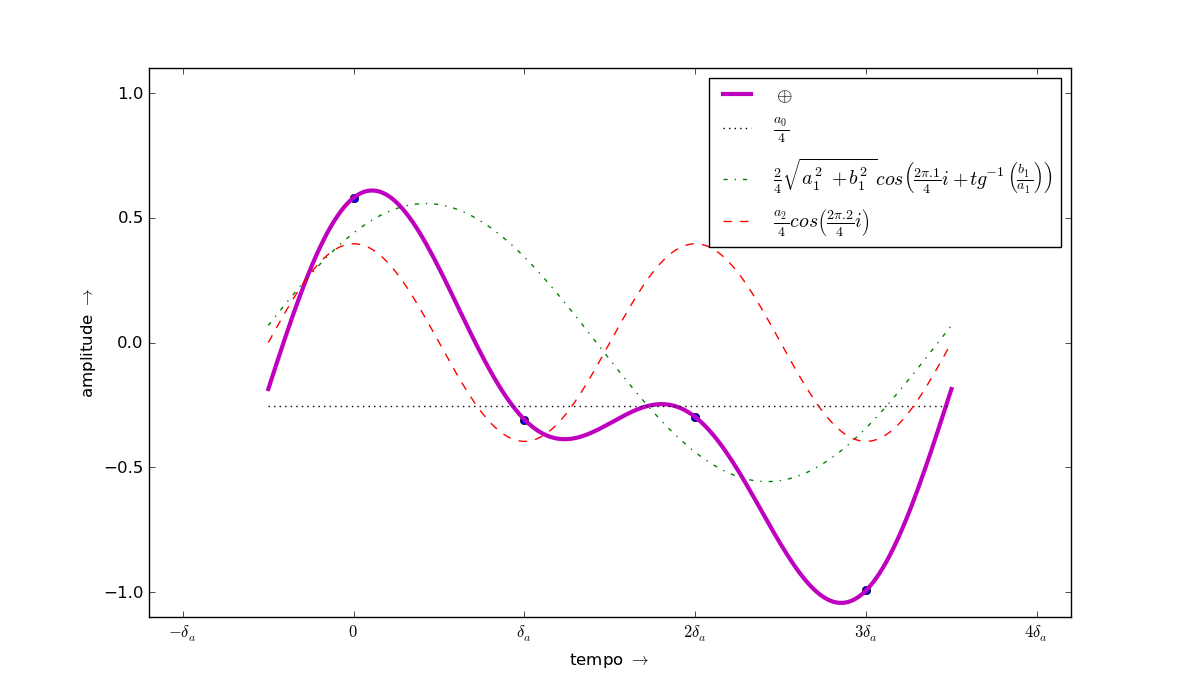
\includegraphics[width=\textwidth]{figuras/amostras4_}
        \label{fig:amostras4}
\end{figure}

\begin{figure}[h!]
    \centering
    \caption{Formas de onda básicas em 4 amostras}
        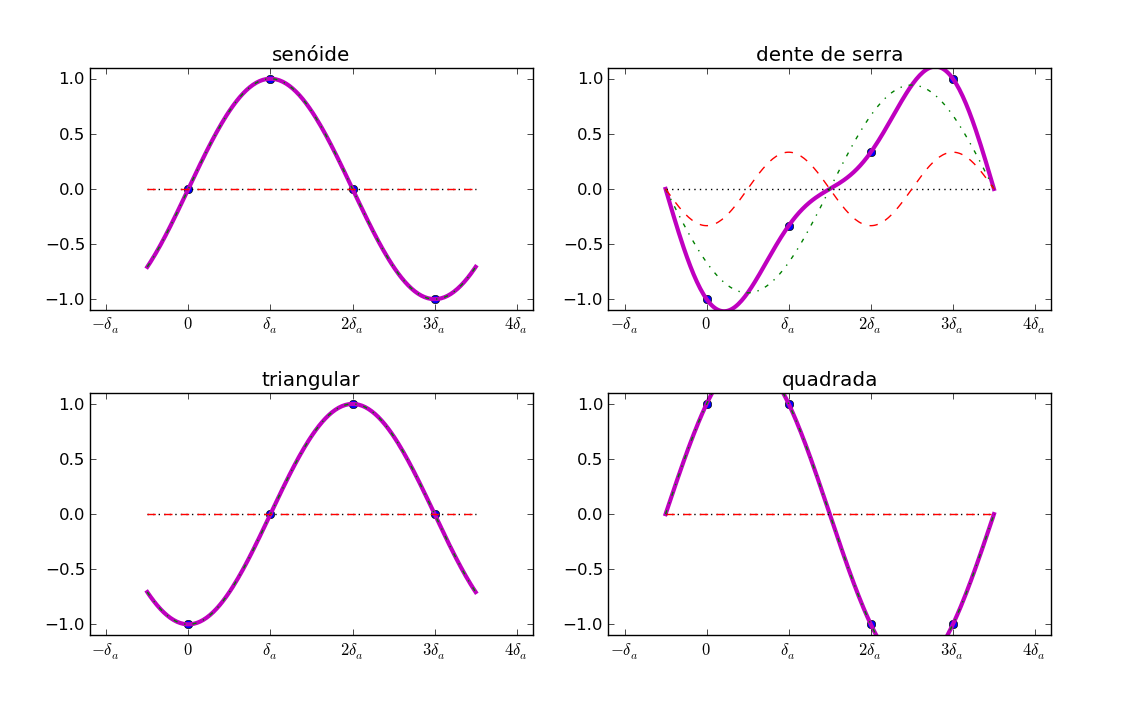
\includegraphics[width=\textwidth]{figuras/amostras4formas}
        \label{fig:formas4}
\end{figure}


A figura ~\ref{fig:amostras6} mostra as decomposições senoidais para o caso de 6 amostras. A figura ~\ref{fig:formas6} decompõe as formas de onda básicas. Note que as ondas se diferenciam espectralmente.

\begin{figure}[h!]
    \centering
    \caption{Componentes frequenciais em 6 amostras}
        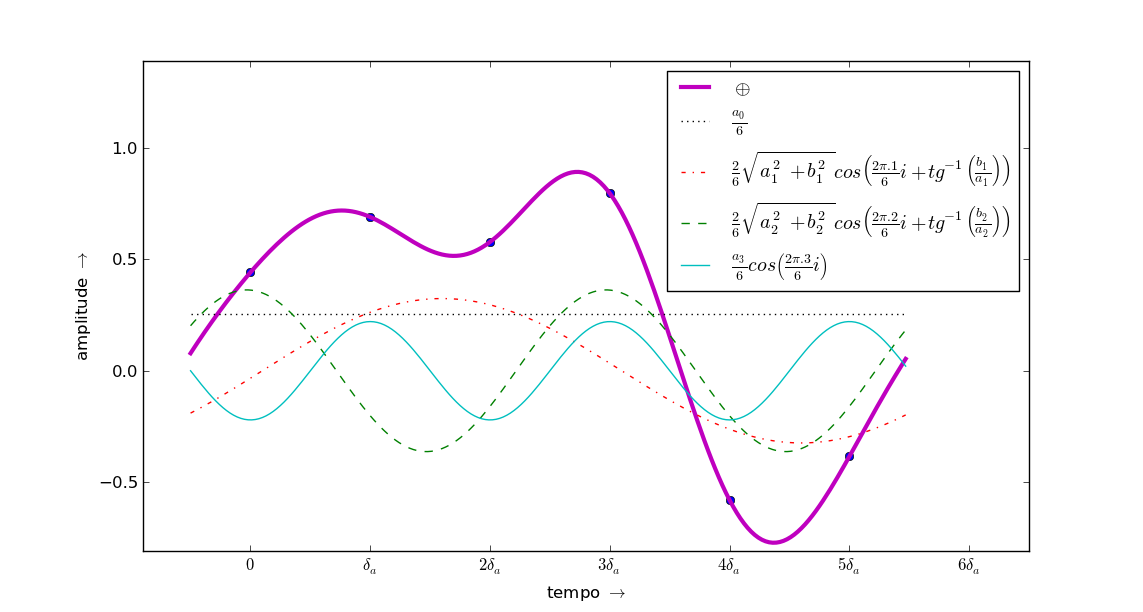
\includegraphics[width=\textwidth]{figuras/amostras6}
        \label{fig:amostras6}
\end{figure}

\begin{figure}[h!]
    \centering
    \caption{Formas de onda básicas em 6 amostras}
        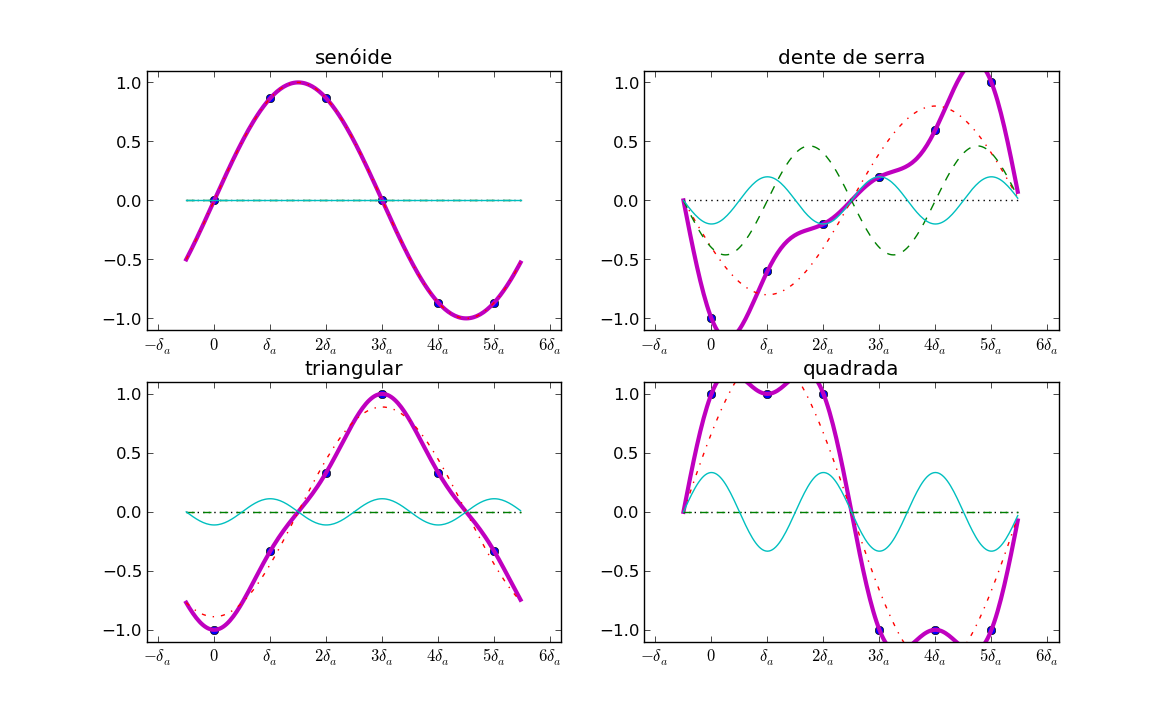
\includegraphics[width=\textwidth]{figuras/amostras6formas_}
        \label{fig:formas6}
\end{figure}

\subsubsection{A nota básica}

Escolhamos $f$ tal que $f$ divide $f_a$   \footnote{Esta escolha facilita as demonstrações pois os períodos são quantidades inteiras de amostras. Transporemos esta limitação na prática com o uso de uma tabela de amostragem ou com o uso direto de funções periódicas,e.g. $t_i=sen(x.i)$}. Uma sequência $T_i$ de amostras sonoras periódicas separadas por $\delta_a=1/f_a$ descreve uma nota musical de frequência $f$ Herz e duração $\Delta$ segundos se possuir a periodicidade $\lambda_f=f_a/f$ e tamanho $f_a . \Delta$:

\begin{equation}
T_i^{f,\; \Delta}=\{t_{i \, \% \lambda_f} \}_0^{f_a . \Delta}=\{t_{i \; \% \left( \frac{f_a}{f} \right) } \}_0^{f_a . \Delta}
\end{equation}

Note que a nota por si só não especifica um tímbre. Mesmo assim, faz-se necessária a escolha de uma forma de onda para que as amostras $t_i$ tenham um valor estabelecido individualmente. Um único período dentre as ondas básicas pode ser utilizado para a especificação da nota da seguinte forma. 

Seja $f$ a frequência da nota, $\delta_f=1/f$ o seu comprimento de onda e $L_i^{f,\, \delta_f} $ a sequência que descreve um período da onda $L_i^f \in \{S_i^f,Q_i^f,T_i^f,D_i^f,R_i^f \}$ (ver equações ~\ref{senoide}, ~\ref{denteDeSerra}, ~\ref{triangular} e ~\ref{quadrada}; $R_i^f$ é uma onda real amostrada),

\begin{equation}
L_i^{f , \delta_f } = \{ l_i^f \}_0^{\delta_f . f_a -1}=\{ l_i^f \}_0^{\lambda_f-1}
\end{equation}

Então a sequência $T_i$ consistirá em uma nota de duração $\Delta$ e frequência $f$ se:

\begin{equation}
T_i^{f,\; \Delta}=\{t_i^f\}_0^{f_a . \Delta}=\{l^f_{i\,\%\left(\frac{f_a}{f}\right)}\}_0^{f_a . \Delta}
\end{equation}

\subsubsection{Usos musicais}


\section{Áudio e Música (deprecated)}

Por razões didáticas, dividimos este capítulo em 4 partes: música em tempo diferido (ou seja, que não é feito em tempo real),
música em tempo real,  música na matéria (suporte físico em hardware) e música no tecido social
(considerando especialmente as mobilizações humanas relacionadas).

Com isso desejamos expor a prática musical através do código
com exemplos reais de aplicação e em uso pelo autor, por membros do LabMacambira.sf.net,
por parceiros, colaboradores e por usuários eventuais das naturezas mais diversas.

  \subsection{Música em Tempo Diferido: Minimum-fi e FIGGUS}

\begin{quotation}
\small
'The increasing dominance of graphic interfaces for music software obscured 
the continuing presence of the command-line tradition, 
the code writer, the hacker. The code writing of deferred time 
computer programming may be assembled out of time order, debugged and optimized.'

\emph{Simon Emmerson, Living electronic music, 2007}
\end{quotation}

A realização musical em tempo diferido é o paradigma inicial da música computacional.
Iniciando com o Music V, a proposta foi depois desenvolvido com o CSound. Pode-se dizer
que até hoje é a forma como compositores usualmente pensam a música: pensando
e escrevendo as estruturas, que depois são executadas por instrumentistas ou aparelhos eletrônicos.

Assim como a composição instrumental permite um trabalho mais minucioso do que
a improvisação instrumental, a realização musical em tempo diferido usualmente permite um
detalhamento maior dos procedimentos do que a realização em tempo real. Por este
mesmo motivo, trataremos inicialmente de dois trabalhos em tempo diferido.
Aliás, como veremos a seguir, as abordagens completam uma base para a música
computacional praticada até os dias de hoje.

O som musical pode ser caracterizado físicamente, e sua síntese digital com base em nossa banda de audição e no teorema de Nyquist, sintetiza uma música amostra por amostra, através de princípios
claros de síntese sonora e organização musical\footnote{Veja no APÊNDICE XX: o \emph{minimum-fi} hi-fi, low-fi, minimum-fi, ou seja,
o mínimo de qualidade para assegurar existência e consistência
da criação}. O segundo, chamado de \emph{FIGGUS} (FInite
Groups in Granular and Unit Synthesis), utiliza os princípios do minimum-fi e constitui
um módulo Python completo, cuja proposta é a utilização de simetrias, através de
permutações e de Teoria de Grupos, para a composição de músicas. Como demonstração
das capacidades do FIGGUS, ele gera um EP\footnote{Extended Play, uma album musical maior que um single mas menor que um LP (Long Play) inteiro} com um único comando. Este é o
\emph{PPEPPS}\footnote{Pure Python EP: Projeto Solvente}, como veremos a seguir.

Desta forma, esta sessão exemplifica e explicita - através de dois exemplos reais - os
princípios do uso de código para a síntese \emph{musical}, desde as amostras
relativas a uma nota com dada frequencia, amplitude e timbre, até a confecção
de uma ferramenta derivada, já incorporando propostas musicais e estruturas
mais elaboradas.

      \subsubsection{Minimum-fi}

Existe uma perene matiz estética e também tecnológica
de realizar uma dada tarefa com \emph{o mínimo} necessário.
Esta matiz é para a música igualmente
fundamental e reconhecida como
princípio de unidade e coerência\footnote{Este princípio tanto é fundamental
que as escolas musicais possuem técnicas específicas, músicas possuem suas
próprias convenções mantidas por toda a sua duração, os arcos mantém características,
enfim, podemos até mesmo concluir que a simetria define o escopo.}. Em código computacional
a empreitada para manifestar este princípio ele próprio de forma mínima
resultou no \emph{minimum-fi.py}, código Python em um único arquivo curto que sintetiza
músicas com segundo as estruturas especificadas em linha\footnote{Em música se fala da \emph{bula} (que equivaleria
às funções em si e das especificações da linguagem) e a partitura ou 'música' propriamente ditas (que equivale à .}.
Na versão atual, de 2012 mas adiantada em 2011, os algorítmos 
em Python propriamente ditos somam 
53 linhas e inclui 5 funções. Com estas funções, estruturas musicais podem 
ser criadas padrão a padrão, nota a nota, amostra por amostra. Na prática e posto em
linguagem cotidiana, resultam em notas que formam
blocos e estruturas hierarquicamente superiores.


Os princípios, bastante simples\footnote{Osvaldo Lacerda, em seu livro \emph{Compendio de Teoria Elementar da Musica} fala das propriedades do som musical de forma equivalente.}, são:
\begin{itemize}
  \item Deve-se ter um mecanismo de síntese sonora que
possibilite a geração de unidades sonoras com diferentes timbres, controle sobre a frequência fundamental e duração específica\footnote{Também entra aqui o volume, mas como o que controlamos de fato é a intensidade relativa entre as notas, resolvemos por bem omitir
esta parte até que fiquem claros os códigos relativos a isso, logo abaixo.}.
  \item Deve-se ser capaz de construir não só unidades sonoras, mas também séries de unidades, sejam sobrepostas (acordes, por exemplo)
  ou justapostas (melodias, por exemplo).
\end{itemize}

Para o primeiro item, se prestam comumente os procedimentos de busca em tabelas/vetores com formas
de ondas em alta resolução (chamado \emph{lookup table}). O procedimento é barato e de qualidade alta
(não acrescentam ruídos relevantes ao sinal).

Para realizarmos a busca de forma eficiente, precisamos de tabelas que contenham cada uma
uma forma de onda. As tradicionais são a senóide e as ondas quadrada, triangular e dente de serra.
Mostramos a seguir estas formas de onda e também uma forma de onda retirada de um som real.

De posse destas formas de onda, A seguir está o procedimento da lookuptable:

\code{Procedimento de Lookup Table}{python_snippets/lookuptable.py}

O primeiro ponto importante é a tabela em si, usualmente unidimensional. É de comum conhecimento que
tabelas com 1024 são mais que suficientes para os usos musicais e a diferença
de qualidade (relação sinal/ruido) não muda consideravelmente com a utilização
de tabelas maiores. A seguir dispomos algumas destas tabelas, mais 
especificamente, dispomos as tabelas para os formatos de onda mais usuais. 

\code{Formas de Onda Tradicionais}{python_snippets/formasDeOnda.py}

Através da utilização do lookup sucessivo (procura-se um valor na primeira tabela
e este valor indica o valor na segunda tabela a ser utilizado), executamos
um waveshaping. Este procedimento é bastante apreciado pela simplicidade e eficácia
na síntese de tímbres diversos e ricos em harmônicos e evolução temporal. Embora
uma explicação exaustiva do waveshaping fuja ao escopo deste trabalho, este
método se caracteriza pela aplicação de uma função não linear ao sinal de entrada.
Neste caso o sinal de entrada é gerado pelo primeiro lookup, a função não linear aplicada
é representada pela segunda tabela e aplicada pelo segundo lookup.

Existem muitas formas de se executar waveshaping, a seguir segue o que usamos no minimum-fi, que se sustenta principalmente por ser leve e simples:

\code{Waveshaping com Lookups sucessivas}{python_snippets/lookup_cruz.py}

O segundo item - dos dois princípios expostos sobre o minimum-fi - presta-se à discretização do espaço musical. Unidades como batidas e notas
tornam mais eficiente a comunicação pois a quantidade
de estruturas sugeridas é maior e as estruturas são mais claras no discreto do que no contínuo~\cite{Roederer}. Roederer chega a
apontar que as próprias notas dos instrumentos musicais são um reflexo de que é mais eficiente
o uso do discreto do que do contínuo para a geração de estruturas musicais.

De fato, unidades bem definidas se mostram úteis na prática musical 
para fazer sequências de unidades, concatená-las. Quando as unidades
são notas, as sequências de unidades justapostas no tempo são melodias ou linhas melódicas. As
sequências sobrepostas no tempo são comumente pensadas como acordes, mas podem ser tidas simplesmente
como sobreposições circunstanciais de duas linhas melódicas. Isso, claro, segundo
a sistematização clássica e usual da música~\cite{Lacerda}\footnote{Vole assinalar aqui que a música do século XX apresentou diversos modelos teóricos que quebram com este entendimento simplificado sobre a música, suas unidades básicas e estruturas relacionadas}.

As duas construções básicas explicitadas a seguir, baseadas na dicotomia melodia/harmonia
(horizontalidade/verticalidade, justaposição/sobreposição), são
as funções \emph{fazSequencia} e \emph{fazAcorde} no minimum-fi. Vale notar elas são absolutamente 
equivalentes em uma análise puramente conceitual, i.e. uma delas pode ser omitida segundo algumas teorizações. Isso fica particularmente óbvio quando se nota que os procedimentos de mixagem e concatenação são
plenamente capazes de realizar o que estas funções realizam. Aliás, as funções nada
mais são do que usos típicos e quase caricatos destes procedimentos: no fazAcorde a mixagem
sobrepõe no tempo todas as unidades, no fazSequencia as unidades são todas juntapostas no tempo.

Como pode-se notar a seguir, as sequências de notas e os acordes, em última instância, são utilizações específicas das 2 funções de síntese sonora explicadas anteriormente: lookup e lookupcruz.

\code{Realização de Sequências de Notas}{python_snippets/fazSequencia.py}

\code{Realização de Acordes de Notas}{python_snippets/fazAcorde.py}

A última das cinco funções utilizadas é uma soma amostra a amostra de dois sons. Para isso,
é necessário completar com zeros a sequência com o menor número de amostras para somar rapidamente:

\code{Somador (função auxiliar)}{python_snippets/somador.py}

Depois disso é usufruir com estruturas criadas. Por exemplo: depois de construidas
algumas tabelas para serem usadas como diferentes timbres, pode-se criar as
escalas completamente simétricas na oitava cromática assim:

\code{Escalas Completamente Simétricas (na grade dos 12 semitons e no âmbito da oitava)}{python_snippets/escalas_simetricas.py}

% escala\_1=range(12) # cromática ascendente sem inclusão da oitava
% escala\_2=range(0,12,2) # tons inteiros
% escala\_3=range(0,12,3) # diminutão
% escala\_4=range(0,12,4) # terças maiores
% escala\_6=range(0,12,6) # trítonos
% \end{python}
% \input{py}

Sendo cada unidade um semitom. Ou seja, cada unidade é o fator que fica presente na conta $f_0 . 2^{(1/12)} . fator $ e resulta na frequência exata da nota relativa a $f_0$ em um sistema temperado ideal.

Podemos também utilizar as usuais
escalas tonais maior e menor natural, harmônica e melódica:

\code{Escalas diatônicas tonais (maiores e menores)}{python_snippets/escalas_Mm.py}

A utilização de intervalos menores que o semitom\footnote{Prática também conhecida
como \emph{microtonalismo}, que gera/utiliza \emph{microtonalidade}.} mostra-se trivial em
nossa implementação. Basta representar sequências de fracionários
que são partes linearmente proporcionais dos semitons ou modificar o fator $f$:

\code{Escalas Microtonais (com quartos e oitavos de tom e intervalos menores)}{python_snippets/escalas_microtonais.py}

Da mesma forma, as triades maiores e menores
são especificadas com simplicidade. Note que aos acordes \emph{diminutão} e
\emph{aumentado} correspodem as mesmas notas das escalas simétricas de terças menores
e maiores respectivamente:

\code{Acordes anotados como listas em python}{python_snippets/acordes.py}


E séries/sequências podem ser anotadas junto a variações:

\code{Séries diversas}{python_snippets/series.py}

Com este arcabouço, o passo seguinte é sintetizar e mixar, resultando
em sequências musicais. A síntese de sequências e acordes são feitos tipicamente
através de comandos desta forma:

\code{Sintetizando sequências e acordes}{python_snippets/seqs_acordes.py}

Já a síntese de estruturas compostas (p.ex. sequências de acordes e sobreposição
de linhas melódicas), são feitas com os recursos usuais da liguagem. Neste caso
usamos listas em Python e implementações em Numpy (mais eficientes em tempo de
execussão e também na simplicidade do código) estão no apêndice. Estes mesmos
procedimentos são praticamente os mesmos em Scilab, C/C++, Javascript, PHP, etc.

A seguir demonstramos para fins didáticos, a construção de acordes periódicos em
python puro\footnote{A implementação não didática destas três linhas de código
podem ser agrupadas em uma só linha.}:

\code{Acordes periódicos}{python_snippets/acordes_periodicos.py}

Em posse destas sequências, acordes e recursos da linguagem,
formamos estruturas hierarquicamente superiores
através da concatenação de estruturas, da mixagem de estruturas, e da amplificação
(ou atenuação) seletiva das mesmas:

\code{Amplificação e mixagem}{python_snippets/amp_mix.py}

Neste ponto, basta criarmos músicas e sequências de interesse estético ou para pesquisa. Dado o ferramental, os encadeamentos dependem de intensões estéticas, entendimentos musicais e estruturas abstratas que mantém a coerência e interesse em uma peça musical. Para o leitor mais interessado, deixamos para o Apêndice X um exemplo de música feita com o minimum-fi. A seguir utilizamos esta base apresentada para sintetizar estruturas musicais e então um EP.

\vspace{10 mm}

        \subsubsection{FIGGUS: FInite Groups in Granular and Unit Synthesis}

Em coerência com os conhecimentos
e tecnologias já apresentados nesta exposição\footnote{Especificamos o arcabouço para geração de sons musicais em unidades
e estruturas compostas logo acima na subsessão sobre o minimum-fi.}, introduzimos agora
um foco especial nas estruturas musicais
desenvolvidas. São elas, inseridas em um momento histórico e
executadas por instrumentos específicos com as técnicas de época,
que constituem uma linguagem musical e músicas propriamente
ditas[ref]. O FIGGUS constitui uma técnica composicional
manifestada em software como ferramenta de síntese de
estruturas musicais por estruturas matemáticas específicas
para representação de simetrias.

Este desenvolvimento foi iniciado em 2006 com o físico-matemático Prof. Adolfo Maia Junior - bem anterior
ao nascimento do minimum-fi - para
tratar de simetrias na música com vistas à composição musical através
de métodos matemáticos\footnote{Duas iniciações científicas trataram do assunto, convenios XXX e YYYY.}. Mais especificamente, a proposta resultou em
um programa voltado para a síntese
granular e síntese de estruturas musicais através de Grupos Algébricos. O nome dado
foi FIGGUS, sigla de FInite Groups in Granular and Unit Synthesis\footnote{Também utilizamos
o nome FIGGS (FInite Group in Granular Synthesis) dado que o termo \emph{unit synthesis} não
é usual na literatura. Posteriormente o primeiro autor deste trabalho recorreu novamente
ao uso do nome FIGGUS. Isso foi motivado principalmente pelo fato de que
o maior uso da técnica é para síntese de estruturas musicais, não para
síntese de amálgamas sonoros (ou timbres mesmo) tipicamente resultantes da síntese granular}.

Na atual reescrita, embora ainda bastante atrás do FIGGUS original quanto
à interface gráfica, a ferramenta opera diretamente em Python puro,
com as biblitecas imbutidas por padrão. Isso permite com que o FIGGUS
sintetize todo um EP usando somente os comandos:

\code{Utilizando o FIGGUS para Sintetizar um EP}{python_snippets/synth_ep.py}

Desta forma, a ferramenta fica muito mais simples para experimentações
e implementações adicionais pois sua utilização se dá através
do próprio código no qual tudo é especificado. Esta abordagem se mostra particularmente
pertinente pois a estagnação do mecanismo de síntese de estruturas musicais
beira a inviabilização do uso artístico ou torna necessário o uso
de recursos externos.
Outro uso pretendido para o FIGGUS
é a síntese de tímbres e amálgamas sonoros através da
Síntese Granular. Embora nosso foco seja outro, cabe algumas breves
palavras sobre o assunto.

A Síntese Granular é uma área bem estabelecida tanto na acústica quanto
na Computação Musical e se caracteriza pela geração de sons bastante curtos
e em quantidade massiva. Tipicamente os sons possuem entre 5 e 40 milissegundos
e a quantidade destes \emph{microsons}\footnote{Grãos sonoros e microsons são jargões
típicos da síntese granular usados para indicar sons com as durações especificadas
no texto.} pode chegar a milhares por segundo. O tratamento específico da
síntese granular foge ao escopo deste trabalho e indicamos ao leitor interessado
os artigos produzidos sobre Síntese Granular e Teoria de Grupos[refs AES e SBCM].
Assim, focamos o texto a seguir em Grupos Finitos e Síntese de Estruturas Musicais.

Nas artes é de comum conhecimento o papel absolutamente central
que as simetrias possuem. Na música, para citar somente alguns exemplos simples,
temos os numerosos estudos de simetrias na música de J. S. Bach, os jogos
de dados de Mozart e os usos recorrentes da proporção áurea na música
de Béla Bártok. Matematicamente, as \emph{simetrias} são descritas por Grupos,
e estes são definidos como sendo um conjunto (chamemos de $G$)
munido de uma operação (seja $\bullet$), formando um grupo $(G,\bullet)$
satisfazendo as seguintes propriedades:

\begin{enumerate}
    \item Fechamento: $\forall \ g_1, g_2  \in G \Rightarrow g_1 \bullet g_2 \in G$
    \item Associatividade: $(g_1 \bullet g_2) \bullet g_3 = g_1 \bullet (g_2 \bullet g_3), \forall \ g_1, g_2, g_3 \in G$
    \item Existência do elemento neutro: $\exists \ e \in G : g \bullet e = e \bullet g = g$
    \item Existência dos inversos: $\forall \ g \in G \ \exists \ g^{-1} : g \bullet g^{-1} = g^{-1} \bullet g = e$
\end{enumerate}

Adicionalmente, vale complementar que se um grupo tiver um número
finito de elementos, ele é dito finito, caso contrário é chamado
infinito. Todos os elementos de um grupo finito são cíclicos pois
operado com si próprio um número suficiente de vezes resulta em si
mesmo. Um grupo é dito comutativo ou abeliano caso a propriedade
comutativa seja satisfeita para todos os elementos:
$\forall \ g_1, g_2 \in G \Rightarrow g_1 \bullet g_2 = g_2 \bullet g_1$.

São numerosas as aplicações de grupos e estes
usos para as artes possam se desenvolver
de diversas formas focadas em simetrias
e com interesse estético, em
nossas pesquisas uma delas se mostrou particularmente coerente
e pertinente: as permutações de unidades sonoras. Primeiro,
através do Teorema de Cayley, todo grupo finito é isomorfo
a um grupo de permutação\footnote{Mais especificamente,
todo grupo é isomorfo a um subgrupo do grupo simétrico agindo
em G.}, i.e. seus elementos são diretamente relacionados
a permutações. Além disso, na música as permutações estão
no núcleo de diversos procedimentos canônicos como a
retrogradação e outras técnicas de variação.

[Expor sobre uma ou duas músicas feitas com o FIGGUS]

No FIGGUS, implementamos o grão sonoro (no caso mais usado
como unidade) como uma classe que possui apenas
os seguintes atributos (e não possui funcões): duração (segundos),
frequência (Hz), timbre (identificador para usar mediante implementações convenientes), intensidade (pico $\in \ [0,1]$), e duração dos fades (in e out em segundos). Aqui a classe:


\code{Grão Sonoro Básico}{python_snippets/fgrao.py}

O FIGGUS funciona com base em uma sequência de grãos posta de antemão
na qual operam as permutações. Além da sequência de grãos,
é conveniente também manter o número de grãos da sequência e uma
lista com os índices dos grãos para executar as operações necessárias para gerarmos as músicas (ver abaixo). A classe utilizada para representar as sequências é assim:

\code{Sequência de Grãos}{python_snippets/fsequencia.py}

Aos grãos em sequência neste ponto são aplicadas permutações.
Para isso é bastante conveniente representar as permutações em classesseparadas e os padrões de aplicação destas permutações para facilitar
desenvolvimentos com clareza. No caso a classe de permutações só possui os parâmetros da permutação em si e do tamando dela (número de elementos que ela utiliza). É conveniente implementar uma tradução da notação cíclica para a notação direta da permutação e é uma das facilidades da implementação por classe que fizemos. A classe do padrão de permutação possui também um período de aplicação da permutação, ou seja, de quantas em quantas leituras da sequência aplicamos a permutação. As classes ficaram assim:

\code{Permutações e Padrões de Permutações}{python_snippets/fpermutacoes.py}

De posse dos grãos, da sequência, das permutações e do padrão de permutações estamos possibilitados de realizar a estrutura musical em si. Bastam adicionalmente, especificar o número desejado de iterações da sequência. Com isso, a sequência de grãos é lida um número de vezes, aplicando as permutações na sequência segundo o padrão de aplicação das pemutações, de forma a resultar em uma sequência sonora musical. Note que se a permutação usar menos elementos que a sequência possui, alguns destes elementos ficarão estáticos nas iterações da sequência no padrão sonoro.

Na síntese do vetor sonoro relacionado, é também crucial estabelecer a taxa de amostragem preterida, como podemos perceber na função de síntese dos vetores, da classe Pattern que cuida desta realização do padrão em si. Deixamos a seguir esta função, de forma que faltará apenas a escrita destes vetores sonoros em arquivo de áudio, como veremos a seguir.

\code{Realização do Padrão Musical}{python_snippets/fpadraosonoro.py}

Em posse não apenas de representações abstratas do padrão musical a ser realizado, mas dos próprios vetores sonoros relacionados à representação digital da música a ser realizada, podemos escrever este vetor como um arquivo de áudio propriamente dito. O mais conveniente neste caso é escrever um arquivo PCM (Pulse Code Modulation) em padrão amplamente utilizado e reconhecido. Ambos os padrões WAV e AIFF satisfazem estes requisitos e escolhemos o WAV por ser o padrão de CDs (Compact Discs) e também o mais utilizado por programas de áudio. Mais especificamente, o padrão de CDs é WAV com 44100 amostras por segundo e 16 bits por amostra\footnote{No formato WAV de CD, cada amostra é representada por uma variável inteira 'signed' de 16 bits.}. As amostras dos vetores sonoros são calculados, por conveniência e por convenção, no âmbito $[-1,1]$ e precisam ser normalizados para o âmbito $[-32767,32768]$ e truncados em números inteiros. Depois disso precisam ser escritos em um arquivo com os bits como na convenção da linguagem C/C++. A bibioteca \emph{struct} cuida dessa escrita do inteiro no formato correto, e a biblioteca \emph{wave} escreve o cabeçalho no formato WAV adequado. Assim, a clase de escrita do vetor sonoro em arquivo comum fica assim:

\code{Escrita do Vetor Sonoro em Arquivo WAV}{python_snippets/fio.py}


  \subsection{Música em Tempo Real: Livecoding e ABeatTracker (ABT)}

Com os avanços computacionais recentes, tornou-se usual a síntese sonora
em tempo real. Com isso, surgiram liguagens dedicadas para o áudio e a música
em sua maioria dedicadas - ou ao menos capacitadas - para o uso 
em tempo de execussão [citar PD, SC, ChucK]. Em outras palavras, estas linguagens
possibilitam que o usuário ouça o resultante sonoro do código utilizado e altere
o código com resultado imediato no processamento e resultado que escuta.

Nesta linha de exploração musical do código, iremos expor a seguir sobre
nossas investidas em \emph{Livecoding} (escrita de código em tempo real
com vistas à performance pública) e o ABeatTracker (uma linguagem por macros
para execussão sonora rítmica em conjunto com instrumentos tradicionais e outras
fontes sonoras/musicais externas).


        \subsubsection{Livecoding}

Recentemente, grupos de ponta em música experimental no mundo todo estão
desenvolvendo apresentações musicais públicas baseadas na escrita
de código ao vivo. Usualmente, se projeta o código para que a audiência possa
ver o que está sendo escrito, no rítmo em que se escreve, e se projeta também
o resultante sonoro por autofalantes.

As motivações para isso são variadas. Expomos a seguir de forma topificada
um condensado do que nos orientou a tal prática. Vale ressaltar que são
motivações igualmente presentes em outros grupos, embora não necessariamente
em todos ou da mesmícima forma.

\begin{itemize}
    \item A performance musical por computador carece de recursos performáticos
    à altura das execussões com instrumentos tradicionais. Os gestos são por demais
    discretos e a concentração do performer é bastante focada na tela do computador.
    \item O feedback auditivo do código projetado permite que o espectador infira
    significados dos códigos. Mesmo que de forma superficial, este recurso do livecoding
    é em muito capaz de desmistificar a programação de computadores, por muito considerada
    completamente intangível.;
    \item O código em si é um recurso poderosíssimo, que permite ao usuário controlar
    os sons produzidos amostra por amostra ou em escalas maiores, como notas, compassos, fraseados
    inteiros ou mesmo em escalas maiores de tempo, como minutos, horas, dias e semanas.
    \item O compartilhamento do código é usual, leve e eficiente como entrega completamente
    aberta da tecnologia relacionada à proposta estética.
\end{itemize}

Desta forma, iniciamos em 2011 uma linha de atuação com Livecoding que resultou em uma performance
no \emph{V Festival Contato}. Utilizamos a linguagem ChucK por apresentar os recursos que
consideramos mais apropriados, embora de forma alguma isso seja consensual na prática atual
de livecoding.

A apresentação contou com recursos adicionais para agregar interesse, como a utilização
do \emph{cowsay} (para enviar mensagens enquanto se desenrolava a música) e trajetórias
de um ponto no fundo do código para sugerir a vertigem do sono REM. Estes recursos
podem ser vistos em uso claramente nos videos demonstrativos [citar videos do vimeo].
As linhas do cowsay e o script em processing relacionados estão no Apêndice XX...

Duas pessoas executaram livecoding simultaneamente. A saber, Vilson Vieira executava
rítmos, batidas bastante marcadas que serviam como base. Renato Fabbri, autor do presente
trabalho, executava linhas fluídas quasi melódicas que formavam arcos maiores. Nos intervalos
das investidas no formato citado, havia interlúdios em que ambos se revesavam com músicas
curtas e inusitadas, como em um duelo[disponibilizar músicas em links e colocar de referencia].

[Colocar os códigos meus e do Vilson e explicar o funcionamento e uso]





      \subsubsection{ABeatTracker (ABT)}
O ABT é uma linguagem/ferramenta que dispara linhas rítmicas através de macros que especificam
as células rítmicas, amostras sonoras que são utilizadas como conteúdo sonoro destas
linhas, modos de leitura destas amostras sonoras, e variáveis randômicas utilizadas
para execussão da linha. Além disso, o ABT dispõe de variáveis globais que podem ser alteradas
a qualquer momento pelo usuário, como BPM, velocidade de leitura das amostras e variáveis
randômicas globais (que se somam às individuais).

Em pouco explicitaremos a forma de utilização do ABT. De antemão, é pertinente apresentar
uma pequena discussão a respeito do que o ABT é considerado e sobre os propósitos desta
ferramenta. Em primeiro lugar, vale manter em mente que o ABT tem um funcionamento específico
que pode transcender o que se conhece por livecoding. As macros pré-estabelecidas engendram um
conjunto de recursos pré-estabelecidos bem definido, o que contrasta com a ideia de uma 'linguagem
de programação' que tenha capacidades mais amplas. De qualquer forma, linguagens com domínios
específicos não são raras e por vezes o ABT foi descrito como uma linguagem.

Sobre os propósitos do ABT, em primeiro lugar ele se dispõe a ser um instrumento computacional
essencialmente rítmico. Junto a esta proposta, vem a necessidade da utilização em conjunto com
outros instrumentos, externos ao ABT, ao computador em que estiver rodando e possivelmente externo
com relação a qualquer computador. Para isso foi elaborado o ABD (ABeatDetector), no qual o usuário
tamborila os rítmos que estiver ouvindo ou imaginando para que o ABT sincronize o pulso e utilize
células rítmicas relacionadas. A análise feita pelo ABD resulta em uma série de rítmos explicitados
por sequências de compassos que encapsulem durações regulares do rítmo tamborilado. Estes rítmos
relacionados ao tamborilar do usuário são chamados de harmônicos e podem ser selecionados
prontamente para o disparo de linhas melódicas.

No Apêndice XX está o manual de utilização do ABT e todo o código do ABT (e do ABD) está
disponivel online (citar repos). Exploramos abaixo detalhes relevantes da implementação,
em especial a forma de funcionamento do ABD.

[códigos-chave e explicações sobre o ABT e o ABD]




  \subsection{Música na Matéria: EKP e AHT}

Embora o foco deste trabalho seja na exploração musical através de códigos (abertos!),
nesta sessão iniciamos uma explicação simples, clara e factual de como estas
investidas transcendem o código e até mesmo a música em si.

Mais relevantes que os desenvolvimentos em si, são as mobilizações criadas nos
entornos e os engajamentos. Isso ficará evidente nas próximas - curtas - sessões
destes desenvolvimentos e resultados.

Aqui apresentamos dois trabalhos que geraram alguma movimentação de pessoas,
resultando em reuniões, desenvolvimentos, pesquisas e apresentações propriamente
ditas. O primeiro utiliza o estado do hardware como entrada, o segundo se trata
de uma mesa escultural para flutuação de origamis que resulta em um instrumento musical
bastante lúdico.


      \subsubsection{Emotional Kernel Panic (EKP)}

Em 2008, colaborando intensamente com o CDTL
(Centro de Desenvolvimento de Tecnologias Livres)\footnote{foi uma associação civil formada e desmembrada em 2008 e sediada em Recife, PE}
foi lançada a ideia de utilizar o estado do sistema operacional - especialmente o kernel linux - para
geração de sons. Surge o Emotional Kernel Panic (EKP) na colaboração excepcional de
Felipe Machado\footnote{Importantíssimo para o desenvolvimento da Cultura Digital no Brasil [citar fontes e programas governamentais]},
Ricardo Brazileiro\footnote{Artivista Digital bastante ativo [citar fontes]} e o primeiro autor do presente trabalho.

Desde o inicio, foram definidos três finalidades
para esta exploração do SO:

[visitar o README do EKP e achar os scripts do Brazileiro sobre o EKP]

\begin{itemize}
    \item Didáticos
    \item Artísticos
    \item Monitoramento do SO
\end{itemize}

Toda a base do EKP está aqui: http://trac.assembla.com/audioexperiments/browser/ekp-base

[Patches desenvolvidos por Brazileiro/Machado e rascunho do EKP-Monitor]

      \subsubsection{AirHackTable}

A AirHackTable é um instrumento musical eletrônico controlado por origamis (dobraduras de papel), construída na forma de uma mesa. Nela, uma rede de coolers reciclados faz flutuar origamis de geometria e cores variadas. Os movimentos dos origamis são captados por webcam e interpretados em tempo real por software de processamento de imagens, gerando padrões que controlam a transformação sonora da música. Dessa forma, pode-se dizer que os sons gerados refletem o voo dos origamis de acordo com suas geometrias (que geram trajetórias de voo caracteristicas).

Na versão atual da AirHacktable, cada cor (vermelho, amarelo, azul, verde, preto, ou branco) controla uma voz, e a posição do origami na mesa modula aspectos do som. Em outras palavras, se o origami está flutuando mais à esquerda, o som sai no canal à esquerda da mesa, e se o origami está mais próximo da câmera, o volume aumenta, e se está mais afastado do operador, o som se torna mais agudo. 

[imagens da AHT e dos patches em operação]

   \subsection{Música no Tecido Social: Sabrina Kawahara, Audioexperiments, EstudioLivre.org, CDTL, juntaDados.org, Devolts.org, MSST, LabMacambira.sf.net}

Esta é uma sessão menor, dedicada a apontar repercussões emergentes destas empreitadas em comunidades diferentes
e então tornar compreensível o desdobramento que estes códigos dedicados à música tiveram em processos sociais
e mobilizações civis.

Grupos foram montados em torno destes desenvolvimentos. Como os propósitos de compartilhamento
e apropriação tecnológica estavam no cerne dos grupos relacionados, as investidas
naturalmente tomaram teores engajados socialmente. A questão do empoderamento das pontas
e da criação de um patrimônio tecnológico da humanidade é consequência quase imediata
das posturas de compartilhamento e apropriação citados.

Discorremos brevemente sobre cada uma das iniciativas citadas:

\begin{itemize}
    \item Sabrina Kawahara
    \item Audioexperiments
    \item Estudiolivre.org
    \item CDTL
    \item JuntaDados.org
    \item Devolts.org
    \item MSST
    \item LabMacambira.sf.net
    \item Outros relacionados: MuSa, Metareciclagem, Submidialogia, Tainã
\end{itemize}


\section{Web}

  Difusão de informação com ênfase na facilitação
  da apropriação de tecnologias e de instancias políticas.

   \subsection{Tecnologias sociais de alta demanda: Sitios, Conteúdos e Articulação}

      \subsubsection{Sítios}

      FDDCA

      Ferramenta de comunicação

      (Cadastro dos pontos?)

      AA, SOS, Catalogo de Ideias, etc

      Meu site pessoal


      \subsubsection{Conteúdos}

      Wiki?

      \subsubsection{Articulação}

      IRC, Emails

\subsection{Disponibilização e desenvolvimento conjunto: wikis, etherpads, AA, Trac, IRC ..}

\subsubsection{Wiki}

\subsubsection{Trac}

\subsubsection{Screencasts - Vimeo}

\subsubsection{AA}

\subsubsection{Audio Experiments (Æ)}

\subsubsection{IRC}

\subsubsection{Etherpads}

\subsubsection{Outras fontes}


\section{Materiais didáticos}

  \subsection{Tutoriais em texto e código: Filtros, Nyquist e plugins LADSPA}

Os vários materiais didáticos produzidos constam no apêndice
deste trabalho. Um único destes será exposto a seguir por sua
capacidade de agregar os conteúdos dos capítulos anterioes:
os tutoriais de filtros e amostragem.

\begin{itemize}
    \item {\bf Tutorial de python para áudio e som}

Este tutorial foi levado para Berlim no LAC 2007 e sofreu melhoras desde entao. Esta
primeira versao ficou resumida em forma de texto no EL\footnote{http://estudiolivre.org/python-e-som-tutorial}. Em 2010
a Associacao Python Brasil escolheu este trabalho, então já mais amadurecido, para ser apresentado no
FISL em Porto Alegre. Como consequencia, foi feita uma série de video-tutoriais bastante utilizados\footnote{http://estudiolivre.org/tiki-index.php?page=Video+Tutoriais}.
Este tutorial foi comentado em listas em que o autor não participa (e outras em que o autor participa).

    \item {\bf Tutoriais de filtros e amostragem via python}

Voltados para explicitar principios fundamentais de áudio, estes tutoriais
são baseados código Python e o equivalente em C. Pequenas explicações são
dadas com o intuito de orientar a exploração inteligente destes \emph{snippets}.

\emph{Teorema de Amostragem}: estes scripts visam a experimentacao inteligente com
o Teorema de Nyquist. (descricao)

\emph{Filtros}: alem da explicitação sobre as diferenças entre filtros FIR e IIR,
duas utilizações clássicas destes filtros estão implementadas: Wavelets (FIR) e Quad (IIR)

Estes códigos podem ser baixados no repositório SVN do AudioExperiments. E os textos estão
na wiki (nos digitais ou EL, recriar pois os CDTL foram apagados)

    \item {\bf Tutorial de plugins lv2}

Dadas as dificuldades que o desenvolvimento dos \emph{plugins} de áudio apresenta,
desenvolvi um tutorial passo a passo com plugins que rodam em todas as etapas.
Ele é baseado em uma interface C++ para este padrão de plugin que eh implementado
em C. Os códigos e os textos estão todos em repositório.

    \item {\bf Microtutoriais Django ~\cite{dmicrotuts}}

Estes 'microtutoriais' são baseados nos conceitos de \emph{scripts mínimos} e
\emph{alterações puntuais}. O primeiro conjunto de microtutoriais é dedicado
a reconstruir o tutorial oficial do django de forma condensada e não prolixa.
O segundo destes conjuntos é dedicado a instrumentalizar de fato o leitor com
o entendimento do funcionamento dos princípios fundamentais deste framework.

    \item {\bf Philosometrics}

Embora este não seja um trabalho didático propriamente dito, ele tem este intuito
no cerne de sua concepção e surgimento. Em decorrência dele, surgiu o  Musimetrics,
o Cinemetrics e o Literametrics. Além disso, ele é um belo exemplo da
utilização das ciências duras para a análise de ciências humanas e foi acolhido
como tal em alguns momentos.

    \item {\bf Carta mídias livres}

Texto criado em decorrência da participação da comissão de seleção no
'Prêmio Mídias Livres', a convite do Ministério da Cultura por 'notório saber'.
Esta carta é um documento único no seu conteúdo, deixando às claras
o conceito de Mídias Livres como mídias não aprisionadas pelo conceito
de propriedade, ou seja, que priorizam a sua livre circulação e a possibilidade
de geração de materiais derivados, assim como sua geração aberta ao colaborativo e comunitário.

    \item {\bf Textos de cunho sociológico, transformador}

Produção mais numerosa que as anteriores, se caracteriza por métodos não convencionais
de abordagem dos assuntos e de escrita. Em especial utiliza-se pseudônimos para
auxiliar a despersonificação, gerando textos menos presos à satisfação da auto-imagem, dente
outras qualidades. A utiliação de psudônimos é um costume muito apreciado em diversos meios,
e as pesquisas tem confirmado as vantagens que a prática apresenta e confirma\footnote{http://disqus.com/research/pseudonyms/}.

O autor destes textos se dá ao direito de não revelar seus psudônimos - embora muitos deles
sejam publicamente conhecidos - para conservar as consequências desta prática na
forma mais pura. Como comprovante desta produção, deixamos uma mensagem sobre a publicação
de textos em mídia impressa com autores internacionais,
confirmando a participação do autor desta dissertação, mas cujo
nome não consta na publicação.

!!!!!!!!!!!!!!!!!!!!!!!!!!!!!!!!!!!!!!!

de      fabi borges catadores@gmail.com por  riseup.net 
responder a     submidialogia@lists.riseup.net
para    submidialogia@lists.riseup.net
data    23 de agosto de 2011 12:26
assunto Re: [submidialogia] livro sub- publicação
lista de e-mails        <submidialogia.lists.riseup.net> Filtrar as mensagens dessa lista de e-mails
enviado por     lists.riseup.net
assinado por    riseup.net
cancelar inscrição      Cancelar a inscrição para essa lista de e-mails
        Importante principalmente porque você frequentemente lê mensagens com esse marcador.
ocultar detalhes 12:26 (6 minutos atrás)
entao, eu fui recebendo textos durante esse tempo,
alguns tao atrazados como dos sem satelites, mas muita gente mandou;

aqui os autores:

os internacionais nao sao muitos, o joni kempf (o que bebe ouro do hardware), o barbrook (futuros imaginarios),
Hamdy heda (da revolucao egipcia), o pedro soller (summerlab), maria llopis (pos porno),  talvez a bronac, nao entregou ainda.

dos brasileiros, renato fabri, ruiz, pasteur, morgana e caio, ju dornelles, mari marcassa, coletivo errorista, adriana velozo-drica, tiago pimentel, felipe fonseca, thiago novaes, lelex, felipe ribeiro(?), maira, verenilde,  bartolina silva, poro, vitoria amaro, fabib (eu),

entao, precisa publicar agora,
uma equipe para publicacao e,,, 

bjs
f

!!!!!!!!!!!!!!!!!!!!!!!!!!!!!!!!!!!!!!!

\end{itemize}

\subsection{Screencasts e outros materiais em video e em texto}

\begin{itemize}
    \item Python para áudio e música
	  Texto - palestras - videos

    \item Canal Macambira
No Macambira estão sendo produzidos materiais em screencasts sobre
diversas cenas de hackeamento.

    \begin{itemize}
	\item Live-Coding
	\item Raspagem de dados
    \end{itemize}
\end{itemize}
